\begin{egBox}{Equivalence Relations and Classes}[eg:22-1]
    Take \( X = \mathbb{R} \).
    We can deem \( x \sim y \) if and only if \( x \) and \( y \) differ by an
    integer.
    E.g.
    \begin{equation*}
        1 \sim 3
        \quad \mathrm{and} \quad 
        \pi \sim \pi + 5    
        \quad \mathrm{and} \quad 
        1 \not\sim 1.5
    \end{equation*}
    This is clearly an equivalence relation.
    Any \( x \) differs with itself by \( 0 \), meaning that \( x \sim x \).
    If \( x \sim y \), it is clear that \( y \sim x \) since differing by an 
    integer is commutative.
    Finally, if \( x \sim y \) and \( y \sim z \), then we get \( x \sim z \)
    since integers are closed via addition/subtraction.

    \baseSkip

    As for the equivalence classes for this given equivalence relation, we see 
    that 
    \begin{equation*}
        [ 1 ]
        =
        \{ \ldots, -2, -1, 0, 1, 2, \ldots \}
        \quad \mathrm{and} \quad 
        [ \pi ]
        =
        \{ \ldots, \pi - 2, \pi - 1, \pi, \pi + 1, \pi + 2 \}
    \end{equation*}

    \baseRule

    Another equivalence relation that we'll frequently look at is one that is 
    associated to a given function \( f: X \rightarrow Y \) between sets.
    It is an equivalence relation on the domain \( X \), where we deem 
    \( x_{ 1 } \sim x_{ 2 } \) if and only if \( f ( x_{ 1 } ) = 
    f ( x_{ 2 } ) \) -- that is, inputs with the same output are deemed 
    equivalent.

    \baseSkip 

    One can see that such a relation, is indeed an equivalence relation.
    We get that \( x \sim x \) immediately due to our function being
    well-defined.
    If \( x \sim y \), it is clear that \( y \sim x \) since equality is 
    itself symmetric.
    Finally, if \( x \sim y \) and \( y \sim z \), then we get \( x \sim z \)
    since equality is again transitive.
\end{egBox}

\begin{egBox}{Quotient Topology}[eg:22-2]
    Let \( I = [ 0, 1 ] \) be the unit interval with the subspace topology.
    Consider the equivalence relation on \( I \) that deems \( 0 \sim 1 \) and
    nothing else extra
    Let \( I^{ * } \) denote the set of all equivalence classes.
    We can think of \( I^{ * } \) as a unit circle \( S^{ 1 } \).

    \baseSkip

    Let us figure out the equivalence classes
    \begin{equation*}
        [ 0 ] = [ 1 ] = \{ 0, 1 \}
        \quad \mathrm{and} \quad 
        [ x ] = \{ x \}
        \text{ where } x \in R \text{ and } x \neq 0, 1
    \end{equation*}
    We can relate \( I \) and \( I^{ * } \) using a special function, denoted 
    \( p \), which sends an element in \( I \) to its corresponding equivalence
    class -- that is, \( p ( x ) = [ x ] \).
    We can see that \( 0 \) and \( 1 \) get sent to the same equivalence class,
    and the rest of the values get sent to their own unique equivalence class.

    \baseSkip 

    In this case, we see that the function \( p \) looks like the "glueing" 
    function.
    Now, if we declare \( V \subset I^{ * } \) to be open, then we would want 
    \( p^{ -1 } ( V ) \) to be open as well -- that is, we want \( p \) to be
    continuous.
    We also want to declare the other implication -- that is, if
    \( p^{ -1 } ( V ) \) is open, then we would want \( V \) to be open in 
    \( I^{ * } \) as well.
    With both of these declaration, we have defined the quotient topology on 
    \( I^{ * } \).
\end{egBox}

\begin{egBox}{Two Special Quotient Maps}[eg:22-3]
    Two special kinds of quotient maps are the \textit{open maps} and the 
    \textit{closed maps}.
    Recall that a map \( f: X \rightarrow Y \) is said to be an \textbf{open
    map} if for each open set \( U \) of \( X \), the set \( f ( U ) \) is open
    in \( Y \).
    If is said to be a \textbf{closed map} if for each closed set \( A \) of 
    \( X \), the set \( f ( A ) \) is closed in \( Y \).

    \baseSkip

    It follows immediately from the definition that if \( p: X \rightarrow Y \)
    is a surjective continuous map that is either open or closed, then \( p \) 
    is a quotient map.

    \baseSkip

    We shall prove the case when \( p \) is an open map.
    Our goal is to show that \( p^{ -1 } ( V ) \) open implies \( V \) is open
    for some \( V \subset Y \).
    Recall that 
    \begin{equation*}
        p^{ -1 } ( V )
        =
        \{ x \in X \mid p ( x ) \in V \}
    \end{equation*}
    Now because \( p \) is surjective, we find that \( p^{ -1 } ( V ) \) will
    contain all the possible values of \( x \) such that every element in 
    \( V \) is hit.
    Thus, it follows that \( p ( p^{ -1 } ( V ) ) = V \).
    Since \( p \) is an open map, and \( p^{ -1 } ( V ) \) is open, it follows
    that \( V \) must be open as well.
    Thus, we have that \( p \) is a quotient map.

    \baseSkip

    We now consider the case when \( p \) is a closed map.
    Our goal is to show that \( p^{ -1 } ( V ) \) open implies \( V \) is open
    for some \( V \subset Y \).
    Since \( p^{ -1 } ( V ) \) is open, it follows that 
    \( X \setminus p^{ -1 } ( V ) \) is closed.
    Notice that 
    \begin{equation*}
        X \setminus p^{ -1 } ( V )
        =
        p^{ -1 } ( Y \setminus V )
    \end{equation*}
    which tells us that \( p^{ -1 } ( Y \setminus V ) \) must be closed as 
    well.
    Since \( p \) is surjective, we see that 
    \( p ( p^{ -1 } ( Y \setminus V ) ) = Y \setminus V \).
    Furthermore, since \( p \) is a closed map, we see that
    \( p^{ -1 } ( Y \setminus V ) \) being closed implies that 
    \( Y \setminus V \) must be closed as well.
    Hence, it follows that \( V \) must then be open.
    Thus, we have that \( p \) is a quotient map.
\end{egBox}

\begin{egBox}{Verifying the Quotient Topology}[eg:22-4]
    Recall that the [\hyperlink{def:22_quotient_top}{quotient topology}], 
    say \( \mathcal{T} \), is defined by letting it consists of those subsets 
    \( U \) of \( A \) such that \( p^{ -1 } ( U ) \) is open in \( X \).
    It is easy to check that \( \mathcal{T} \) is a topology.
    The sets \( \emptyset \) and \( A \) are open since we have that 
    \( p^{ -1 } ( \emptyset ) = \emptyset \) and \( p^{ 1 } ( A ) = X \) -- both
    of which are open in \( X \).
    We have that arbitrary unions of open sets in \( A \) still remain open
    since
    \begin{equation*}
        p^{ -1 } \left( \bigcup_{ i \in I } U_{ i } \right) 
        =
        \bigcup_{ i \in I } p^{ -1 } ( U_{ i } )
    \end{equation*}
    Lastly, we have that finite intersections of open sets in \( A \) also
    remain open since
    \begin{equation*}
        p^{ -1 } \left( \bigcap_{ i = 1 }^{ n } U_{ i } \right)
        =
        \bigcap_{ i = 1 }^{ n } p^{ -1 } ( U_{ i } )
    \end{equation*}
\end{egBox}

\begin{egBox}{Open maps and Quotient Maps}[eg:22-5]
    We examine the function from \( \mathbb{R} \) into the unit circle
    \( S^{ 1 } \) (thought of as the subspace of \( \mathbb{R}^{ 2 } \) defined
    by \( x^{ 2 } + y^{ 2 } = 1 \)) given below:
    \begin{equation*}
        p: \mathbb{R} \rightarrow S^{ 1 }
        \quad \mathrm{where} \quad 
        p ( t )
        =
        ( \cos ( 2 \pi t ), \sin ( 2 \pi t ) )
    \end{equation*}
    One can see clearly that \( p \) is an open map.
    On top of that, we can also see that \( p \) is both surjective and 
    continuous.
    Thus, we have that \( p \) is a quotient map by the 
    [\hyperlink{eg:22-3}{third example}].
\end{egBox}

\begin{egBox}{Equivalent Quotient Spaces}[eg:22.6]
    Let \( \mathbb{R}^{ * } \) be the quotient space determined by the following
    equivalence relation on \( \mathbb{R} \):
    \begin{equation*}
        x \sim y
        \iff 
        x - y \in \mathbb{Z}
    \end{equation*}
    We want to show that \( R^{ * } \) is homeomorphic to the unit circle 
    \( S^{ 1 } \).

    \baseSkip

    To do so, we shall consider the function
    \begin{equation*}
        p: \mathbb{R} \rightarrow S^{ 1 }
        \quad \mathrm{where} \quad 
        p ( t )
        =
        ( \cos ( 2 \pi t ), \sin ( 2 \pi t ) )
    \end{equation*}
    which we previously showed was a quotient map.
    If we can show that the given equivalence relation on \( \mathbb{R} \)
    is equivalent to the equivalence relation on \( \mathbb{R} \) using \( p \)
    (that is, \( x \sim y \iff p ( x ) = p ( y ) \)),
    then we have that by the theorem about equivalent quotient spaces that 
    \( S^{ 1 } \) is homeomorphic to the quotient space of \( \mathbb{R} \).

    \baseSkip

    To show that these two equivalence relations are equivalent, it suffices to
    show that two elements being similar via the equivalence relation using
    \( p \) must also be similar via the equivalence relation given to us, and 
    vice-versa. 
    Indeed, we see this to be the case since both of the components of \( p \) 
    have a period of \( 1 \).
    Thus, we have that \( p ( x ) = p ( y ) \) when \( x \) and \( y \) are some
    multiple of the period away from each other, which is some integer away 
    from each other -- that is, it must be the case that \( x - y \in 
    \mathbb{Z} \).

    \baseSkip

    Hence, we end up getting that \( S^{ 1 } \) to be homeomorphic to 
    \( \mathbb{R}^{ * } \).
\end{egBox}

\begin{egBox}{1 (Munkres)}[eg:22.7]
    Let \( X \) be the subspace \( [ 0, 1 ] \cup [ 2, 3 ] \) of 
    \( \mathbb{R} \), and let \( Y \) be the subspace \( [ 0, 2 ] \) of 
    \( \mathbb{R} \).
    The map \( p: X \rightarrow Y \) defined by
    \begin{equation*}
        p ( x )
        =
        \begin{cases} 
            x \quad & x \in [ 0, 1 ]
            \\ 
            x - 1 \quad & x \in [ 2, 3 ]
        \end{cases}
    \end{equation*}
    is readily seen to be surjective, continuous, and closed.
    Thus, it follows that \( p \) is a quotient.

    \baseSkip

    However, \( p \) is not an open map since the image of the open set
    \( [ 0, 1 ] \) of \( X \) is not open in \( Y \) (there is no open
    interval in \( \mathbb{R} \) that intersects with \( Y \) to get 
    \( [ 0, 1 ] \)).

    \baseSkip

    Now notice that if \( A \) is the subspace \( [ 0, 1 ) \cup [ 2, 3 ] \), 
    then the map \( q: A \rightarrow Y \) obtained by restricting \( p \) is 
    continuous and surjective, but \textit{not} a quotient map;
    the set \( [ 2, 3 ] \) is open in \( A \) and is saturated with respect to
    \( q \), but its image is not open in \( Y \).
\end{egBox}

\begin{egBox}{2 (Munkres)}[eg:22.8]
    Let \( \mathrm{proj}_{ 1 } : \mathbb{R} \times \mathbb{R} \rightarrow 
    \mathbb{R} \) be the projection onto the first coordinate; then 
    \( \mathrm{proj}_{ 1 } \) is clearly surjective and continuous.
    Furthermore, we see that \( \mathrm{proj}_{ 1 } \) is an open map; for if
    \( U \times V \) is a nonempty basis element for 
    \( \mathbb{R} \times \mathbb{R} \), then 
    \( \mathrm{proj}_{ 1 } ( U \times V ) = U \) is open in \( \mathbb{R} \).
    Thus, it follows that \( \mathrm{proj}_{ 1 } \) carries open sets of 
    \( \mathbb{R} \times \mathbb{R} \) to open sets of \( \mathbb{R} \).
    
    \baseSkip

    However, \( \mathrm{proj}_{ 1 } \) is not a closed map.
    The subset 
    \begin{equation*}
        C = \{ x \times y \mid x y = 1 \}
    \end{equation*}
    of \( \mathbb{R} \times \mathbb{R} \) is closed, but 
    \( \mathrm{proj}_{ 1 } ( C ) = \mathbb{R} \setminus \{ 0 \} \), which is
    not closed in \( \mathbb{R} \).

    \baseSkip

    Notice that if \( A \) is the subspace of \( \mathbb{R} \times \mathbb{R} \)
    that is the union of \( C \) and the origin \( \{ 0 \} \), then the map
    \( q: A \rightarrow \mathbb{R} \) obtained by restricting 
    \( \mathrm{proj}_{ 1 } \) is continuous and surjective, but it is still not
    a quotient map; for the one-point set \( \{ 0 \} \) is open in \( A \) and
    is saturated with respect to \( q \), but its image is not open in
    \( \mathbb{R} \).
\end{egBox}

\begin{egBox}{3 (Munkres)}[eg:22.9]
    Let \( p \) be the map of the real line \( \mathbb{R} \) onto the
    three-point set \( A = \{ a, b, c \} \) defined by 
    \begin{equation*}
        p ( x )
        =
        \begin{cases} 
            a \quad & x > 0
            \\ 
            b \quad & x < 0
            \\ 
            c \quad & x = 0
        \end{cases}
    \end{equation*}
    We can see that the quotient topology on \( A \) induced by \( p \) is the
    one indicated in Figure (\ref{fig:22-9})

    \begin{figure}[H]
        \centering
        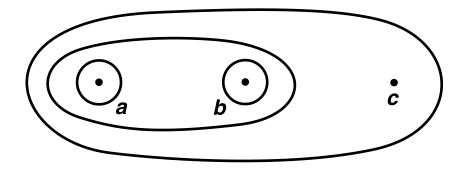
\includegraphics[ width = 0.6\linewidth ]{figures/Section 22/eg22-9.jpg}
        \caption{The quotient topology on \( A \) induced by \( p \)}
        \label{fig:22-9}
    \end{figure}
\end{egBox}

\begin{egBox}{4 (Munkres)}[eg:22.10]
    Let \( X \) be the closed unit ball
    \begin{equation*}
        \{ x \times y \mid x^{ 2 } + y^{ 2 } \leq 1 \}
    \end{equation*}
    in \( \mathbb{R}^{ 2 } \), and let \( X^{ * } \) be the partition of \( X \)
    consisting of all the one-point sets \( \{ x \times y \} \) for which
    \( x^{ 2 } + y^{ 2 } < 1 \), along with the set 
    \( S^{ 1 } = \{ x \times y \mid x^{ 2 } + y^{ 2 } = 1 \} \).

    \baseSkip

    Typical saturated open sets in \( X \) are pictured by the shaded regions 
    in Figure (\ref{fig:22-10}). 
    One can show that \( X^{ * } \) is homeomorphic with the subspace of 
    \( \mathbb{R}^{ 3 } \) called the \textbf{unit 2-sphere}, defined by
    \begin{equation*}
        S^{ 2 } 
        =
        \{ ( x, y, z ) \mid x^{ 2 } + y^{ 2 } + z^{ 2 } = 1 \}
    \end{equation*}

    \begin{figure}[H]
        \centering
        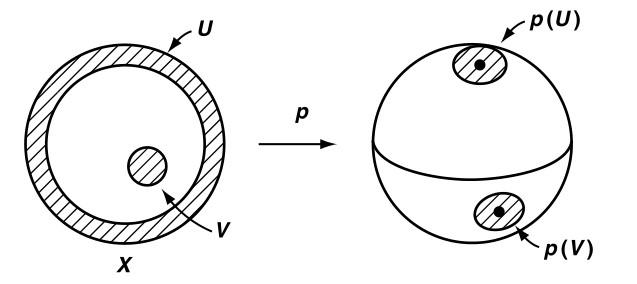
\includegraphics[ width = 0.6\linewidth ]{figures/Section 22/eg22-10.jpg}
        \caption{Typical saturated open sets in \( X \)}
        \label{fig:22-10}
    \end{figure}
\end{egBox}